\documentclass[12pt]{article}



%%%%%%%%%%%%%%%%%%%%%%%%%%%%%%%%%%%%%%
% Metainformation
%%%%%%%%%%%%%%%%%%%%%%%%%%%%%%%%%%%%%%
\newcommand{\trauthor}{Leopold Lemmermann}
\newcommand{\trtype}{Paper}
\newcommand{\trtitle}{Image Captioning}
\newcommand{\trdate}{\today}



%%%%%%%%%%%%%%%%%%%%%%%%%%%%%%%%%%%%%%
% Language
%%%%%%%%%%%%%%%%%%%%%%%%%%%%%%%%%%%%%%
\usepackage[english]{babel}
\selectlanguage{english}



%%%%%%%%%%%%%%%%%%%%%%%%%%%%%%%%%%%%%%
% Bind packages
%%%%%%%%%%%%%%%%%%%%%%%%%%%%%%%%%%%%%%
\usepackage{acronym}                    % Acronyms
\usepackage{algorithmic}                % Algorithms and Pseudocode
\usepackage{algorithm}                  % Algorithms and Pseudocode
\usepackage{amsfonts}                   % AMS Math Packet (Fonts)
\usepackage{amsmath}                    % AMS Math Packet
\usepackage{amssymb}                    % Additional mathematical symbols
\usepackage{amsthm}
\usepackage{booktabs}                   % Nicer tables
% \usepackage[font=small,labelfont=bf]{caption} % Numbered captions for figures
\usepackage{color}                      % Enables defining of colors via \definecolor
\definecolor{uhhRed}{RGB}{254,0,0}      % Official Uni Hamburg Red
\definecolor{uhhGrey}{RGB}{122,122,120} % Official Uni Hamburg Grey
\usepackage{fancybox}                   % Gleichungen einrahmen
\usepackage{fancyhdr}                   % Packet for nicer headers

%\usepackage[outer=3.35cm]{geometry}    % Type area (size, margins...) !!!Release version
%\usepackage[outer=2.5cm]{geometry}     % Type area (size, margins...) !!!Print version
%\usepackage{geometry}                  % Type area (size, margins...) !!!Proofread version
\usepackage[outer=3.15cm]{geometry}     % Type area (size, margins...) !!!Draft version
\geometry{a4paper,body={5.8in,9in}}

\usepackage{graphicx}                   % Inclusion of graphics
%\usepackage{latexsym}                  % Special symbols
\usepackage{longtable}                  % Allow tables over several pages
\usepackage{listings}                   % Nicer source code listings
\usepackage{multicol}                   % Content of a table over several columns
\usepackage{multirow}                   % Content of a table over several rows
\usepackage{rotating}                   % Alows to rotate text and objects
\usepackage[hang]{subfigure}            % Allows to use multiple (partial) figures in a fig
%\usepackage[font=footnotesize,labelfont=rm]{subfig}  % Pictures in a floating environment
\usepackage{tabularx}                   % Tables with fixed width but variable rows
\usepackage{url,xspace,boxedminipage}   % Accurate display of URLs



%%%%%%%%%%%%%%%%%%%%%%%%%%%%%%%%%%%%%%
% Configuration
%%%%%%%%%%%%%%%%%%%%%%%%%%%%%%%%%%%%%%
\hyphenation{whe-ther}                  % Manually use: "\-" in a word: Staats\-ver\-trag

%\lstloadlanguages{C}                   % Set the default language for listings
\DeclareGraphicsExtensions{.pdf,.svg,.jpg,.png,.eps} % first try pdf, then eps, png and jpg
\graphicspath{{./src/}}                 % Path to a folder where all pictures are located
\pagestyle{fancy}                       % Use nicer header and footer

% Redefine the environments for floating objects:
\setcounter{topnumber}{3}
\setcounter{bottomnumber}{2}
\setcounter{totalnumber}{4}
\renewcommand{\topfraction}{0.9}        %Standard: 0.7
\renewcommand{\bottomfraction}{0.5}     %Standard: 0.3
\renewcommand{\textfraction}{0.1}       %Standard: 0.2
\renewcommand{\floatpagefraction}{0.8}  %Standard: 0.5

% Tables with a nicer padding:
\renewcommand{\arraystretch}{1.2}



%%%%%%%%%%%%%%%%%%%%%%%%%%%%%%%%%%%%%%
% Additional 'theorem' and 'definition' blocks
%%%%%%%%%%%%%%%%%%%%%%%%%%%%%%%%%%%%%%
\theoremstyle{plain}
\newtheorem{theorem}{Theorem}[section]
\newtheorem{axiom}{Axiom}[section]
%Usage:%\begin{axiom}[optional description]%Main part%\end{fakt}

\theoremstyle{definition}
\newtheorem{definition}{Definition}[section]

%Additional types of axioms:
\newtheorem{lemma}[axiom]{Lemma}
\newtheorem{observation}[axiom]{Observation}

%Additional types of definitions:
\theoremstyle{remark}
\newtheorem{remark}[definition]{Remark}



%%%%%%%%%%%%%%%%%%%%%%%%%%%%%%%%%%%%%%
% Abbreviations and mathematical symbols
%%%%%%%%%%%%%%%%%%%%%%%%%%%%%%%%%%%%%%
\newcommand{\modd}{\text{ mod }}
\newcommand{\RS}{\mathbb{R}}
\newcommand{\NS}{\mathbb{N}}
\newcommand{\ZS}{\mathbb{Z}}
\newcommand{\dnormal}{\mathit{N}}
\newcommand{\duniform}{\mathit{U}}

\newcommand{\erdos}{Erd\H{o}s}
\newcommand{\renyi}{-R\'{e}nyi}



%%%%%%%%%%%%%%%%%%%%%%%%%%%%%%%%%%%%%%
% Document:
%%%%%%%%%%%%%%%%%%%%%%%%%%%%%%%%%%%%%%
\begin{document}
\renewcommand{\headheight}{14.5pt}

\fancyhead{}
\fancyhead[CO]{\trtitle}



%%%%%%%%%%%%%%%%%%%%%%%%%%%%%%%%%%%%%%
% Cover
%%%%%%%%%%%%%%%%%%%%%%%%%%%%%%%%%%%%%%
\title{\trtitle\\[0.3cm]{\normalsize\trtype}}
\author{\trauthor}
\date{\trdate}
\maketitle

\thispagestyle{empty}

\begin{center}
    \includegraphics[width=0.2\textwidth]{src/wtmicon.pdf}
\end{center}

\begin{abstract}
 This paper is about image captioning. We discuss the current state of the art and overview the most important methods. We present our results of experiments with different encoder and decoder models. We use the flickr8k dataset and evaluate the models using the BLEU score. We discuss the results and give an outlook on future work.
\end{abstract}

\tableofcontents
\newpage
\pagenumbering{arabic}



%%%%%%%%%%%%%%%%%%%%%%%%%%%%%%%%%%%%%%
% Content (Outline_Lemmermann_Leopold_TITLE)
%%%%%%%%%%%%%%%%%%%%%%%%%%%%%%%%%%%%%%
\section{Introduction}
\label{sec:introduction}

Image captioning involves generating textual descriptions of given images. It is a difficult problem because it combines the visual and textual domains. In recent years, deep learning has revolutionized the field of image captioning.

This paper presents an overview of the most essential methods in image captioning and some of our results.

Image captioning is a complex and interdisciplinary task bridging computer vision (CV) and natural language processing (NLP). The objective is to generate natural, descriptive sentences for images, which involves detecting and interpreting visual elements and their relationships within scenes. Recent advancements leverage deep learning, particularly Convolutional Neural Networks (CNNs) for feature extraction and Recurrent Neural Networks (RNNs), especially Long Short-Term Memory (LSTM) networks, for sequential language generation. For instance, models such as "Show and Tell" \cite{Vinyals:2015} and "Show, Attend, and Tell" \cite{Xu} utilize CNN-RNN architectures, with the latter integrating attention mechanisms to enhance focus on specific image regions, thereby improving caption relevance and accuracy.

Image captioning models are typically evaluated using metrics like BLEU, METEOR, and CIDEr, which assess linguistic similarity to human references. While these metrics are widely accepted, considering the quality of image captions remains challenging due to the subjective nature of language generation. Additionally, methods like Reinforcement Learning (RL) have been explored to optimize these models directly on evaluation metrics, addressing issues such as exposure bias by aligning training and inference methods more closely \cite{Rennie}.

Recent innovations in diverse decoding strategies, like Diverse Beam Search, aim to overcome the tendency of beam search to produce near-duplicate captions by enhancing variability without sacrificing quality. Diverse Beam Search ensures that generated captions capture a broader range of plausible descriptions, reflecting the inherent ambiguity in image captioning tasks \cite{Vijayakumar}.



\section{Methods}
\label{sec:methods}

We present the dataset, the encoder-decoder architecture, the encoder models, the decoder models, and the evaluation metrics.

\subsection{Dataset}
\begin{figure}[H]
    \centering
    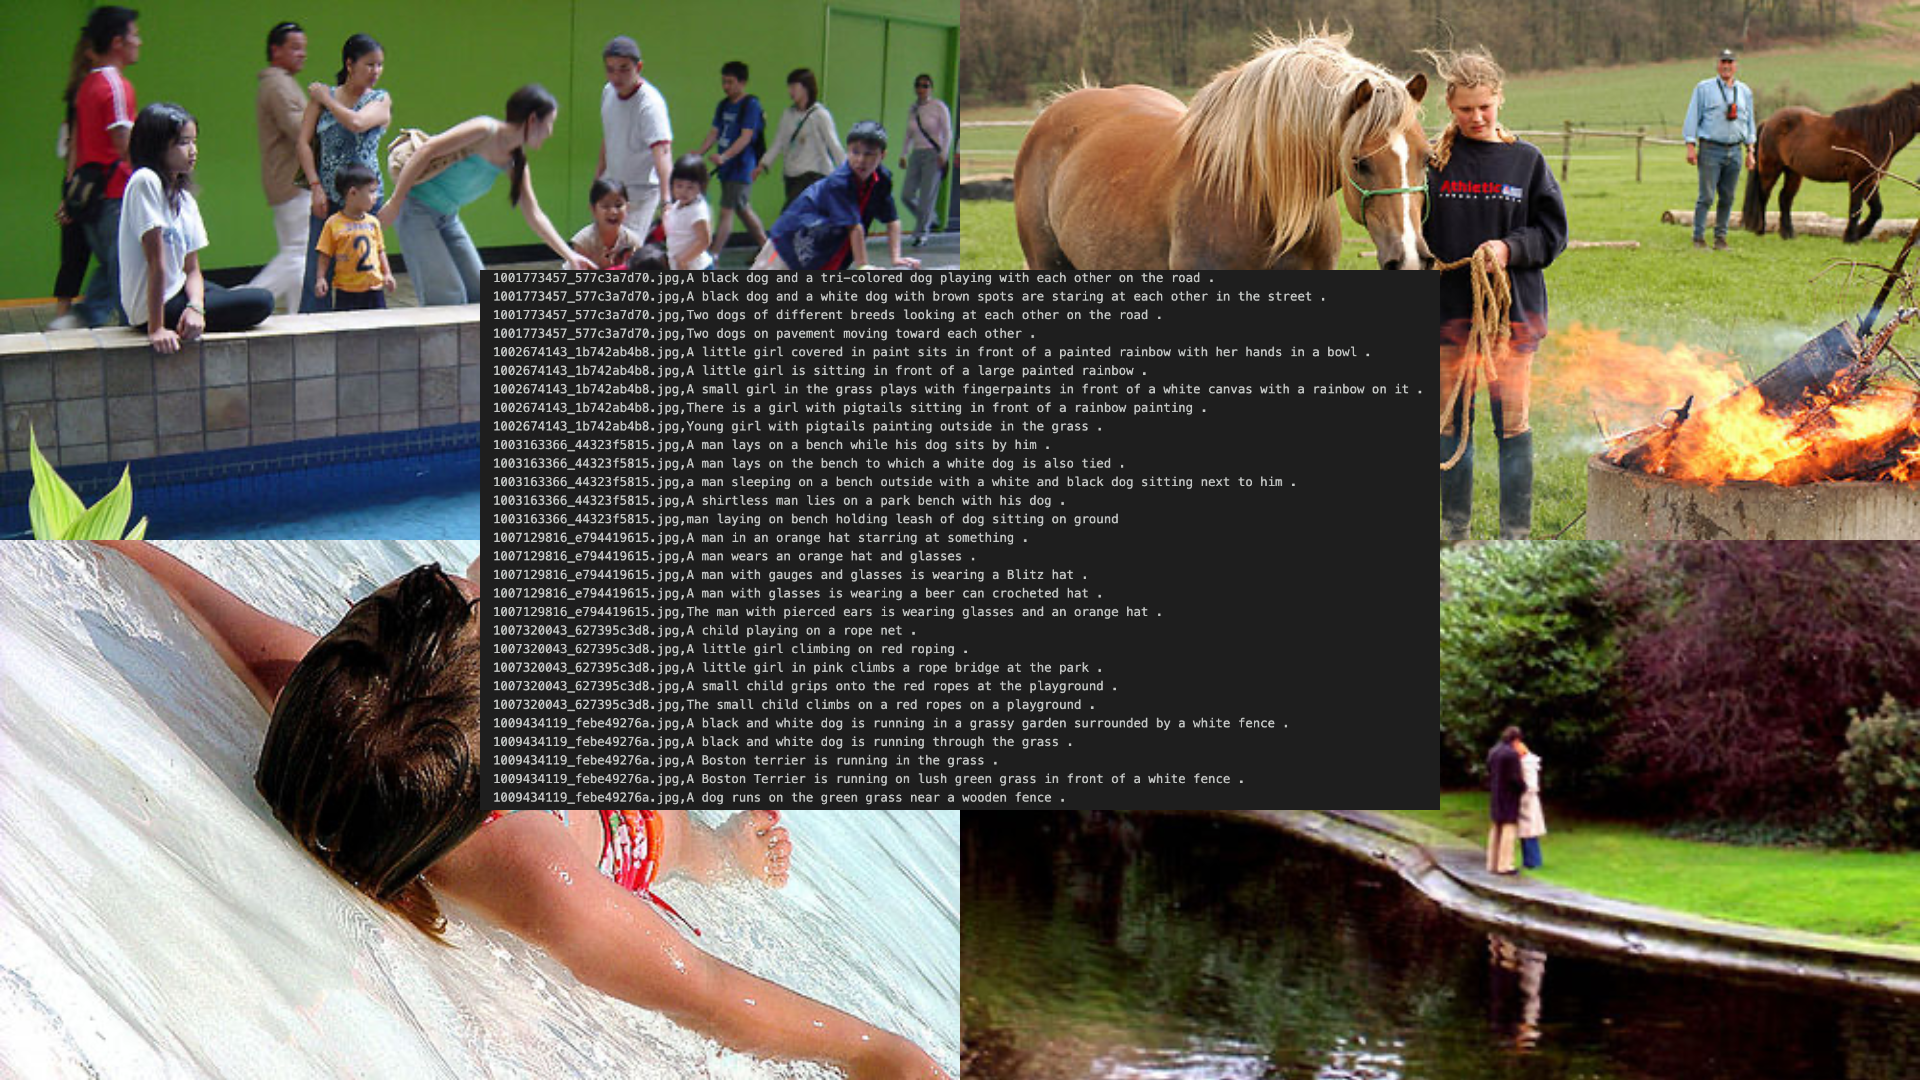
\includegraphics[width=0.8\textwidth]{src/flickr8k.png}
    \caption{Example images and captions from the flickr8k dataset.}
    \label{fig:flickr8k}
\end{figure}
We focused on the flickr8k dataset, which consists of 8,000 images, each with five reference captions. The images are diverse and contain a wide range of objects and scenes. This dataset is commonly used for image captioning research due to its quality and limited size. The captions are relatively short and straightforward, making them easier to generate.
\par Other commonly used datasets are flickr30k and MS COCO, but these datasets are larger and cannot be processed due to our limited computational resources.

\subsection{Encoder-Decoder Architecture}
\begin{figure}[H]
    \centering
    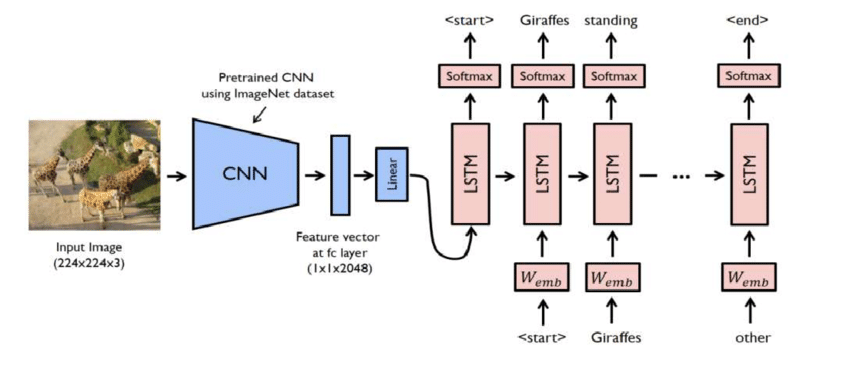
\includegraphics[width=0.8\textwidth]{src/encoder-decoder.png}
    \caption{A Survey on Various Deep Learning Models for Automatic Image Captioning \cite{gaurav}}
    \label{fig:encoder-decoder}
\end{figure}
Usually, an encoder-decoder architecture is used to achieve image captioning. The encoder is a convolutional neural network (CNN) that extracts features from the image. The decoder is a recurrent neural network (RNN) that generates the caption word by word.

\subsection{Encoder Models}
We experimented with two different models for encoding images: ResNet-50 and VGG-16.
\par ResNet-50 is a deep residual network that is widely used for image classification. It has 50 layers and uses skip connections to avoid the vanishing gradient problem. It was introduced in \cite{he}.
\par VGG-16 is a deep convolutional neural network that was developed by the Visual Geometry Group at the University of Oxford. It has 16 layers and is known for its simplicity and effectiveness. It was introduced in \cite{simonyan}.

\subsection{Decoder Models}
We experimented with two different models for decoding captions: GRU and LSTM.
\par Gated Recurrent Units (GRUs) are a type of RNN that is similar to LSTMs but has fewer parameters. They are easier to train and faster to compute. They were introduced in \cite{cho}.
\par Long Short-Term Memory (LSTM) networks are a type of RNN that is designed to avoid the vanishing gradient problem. They have a cell state that can store information over long sequences. They were introduced in \cite{hochreiter}.

\subsection{Evaluation Metrics}
The accuracy of image captioning is commonly measured using BLEU or CIDEr scores.
\par BLEU is a precision-based metric that compares n-grams in the generated caption to those in the reference captions. It ranges from 0 to 1, with higher values indicating better performance. It was introduced in \cite{papineni}.
\par CIDEr is a recall-based metric that compares the generated caption to the reference captions using cosine similarity. It ranges from 0 to 1, with higher values indicating better performance. It was introduced in \cite{vedantam}.
\par For simplicity, we are only using the BLEU score in our experiments.



\section{Approach}
\label{sec:approach}

Our approach begins with data preprocessing, followed by model training and evaluation.

\subsection{Data Preprocessing}
\par We preprocess the images by resizing them to 224x224 pixels and normalizing the pixel values and encoding them to tensors of the dimension (224, 224, 3).
\par We create a vocabulary of words and map each word to an index.
\par We preprocess the captions by tokenizing them, converting them to lowercase, and padding them to a fixed length. Then we encode them using the vocabulary and convert them to one-dimensional tensors with a specified max\_length.

\subsection{Model Training}

\subsection{Model Evaluation}


\section{Results}



\section{Results}
\label{sec:results}

Comparison of different models, evaluation, and discussion.

\section{Conclusion}
\label{sec:concl}

Summary of the results, future work, and open questions.



%%%%%%%%%%%%%%%%%%%%%%%%%%%%%%%%%%%%%%
% References
%%%%%%%%%%%%%%%%%%%%%%%%%%%%%%%%%%%%%%
\newpage
\thispagestyle{empty}

\nocite{*}
\bibliographystyle{apalike}
\bibliography{bib}

\end{document}